\documentclass[problems]{esg8022pset} 
\usepackage{amsmath}
\usepackage{amssymb}
\usepackage{enumerate}
\usepackage{graphicx}
\usepackage{hyperref}
\usepackage{mathtools}
\usepackage[per-mode=symbol]{siunitx} %If this line is giving you trouble, try replacing per-mode with per
%use inter-unit-separator={}\cdot{} ?
\providecommand{\uvec}[1]{{\hat{\bf{#1}}}}
\usepackage{pgf,tikz}
\usetikzlibrary{arrows}
\usepackage{wasysym}
\usepackage{subfig}
\makeatletter
\newcommand{\interitemtext}[1]{%
  \begin{list}{}
   {\itemindent=0mm\labelsep=0mm
   \labelwidth=0mm\leftmargin=0mm
   \addtolength{\leftmargin}{-\@totalleftmargin}}
    \item #1
  \end{list}
}
\makeatother
\renewcommand{\d}{\,d}
\providecommand{\norm}[1]{\lVert#1\rVert}

\newcommand{\Kgrad}{\left(\hat{x} \frac{\partial}{\partial x} + \hat{y} \frac{\partial}{\partial y} + \hat{z} \frac{\partial}{\partial z}\right)}
\newcommand{\Kdiv}[6]{{#4}\left(\frac{\partial {#1}}{\partial x} {#5} \frac{\partial {#2}}{\partial y} {#6}\frac{\partial #3}{\partial z} \right)}
\newcommand{\KKdiv}[6]{{#4}\left(\frac{\partial}{\partial x}{#1} {#5} \frac{\partial}{\partial y}{#2} {#6}\frac{\partial}{\partial z}{#3} \right)}
\newcommand{\dx}{\frac{\partial}{\partial x}}
\newcommand{\dy}{\frac{\partial}{\partial y}}
\newcommand{\dz}{\frac{\partial}{\partial z}}
\newcommand{\dtheta}{\frac{\partial}{\partial \theta}}
\newcommand{\dr}{\frac{\partial}{\partial r}}

\AtBeginDocument{%
  % Apologies to any future editor on the inconsistencies in TeX code and the unnecessary braces.  I'm aggregating previously typeset problems, and didn't think it worth my time to improve the quality of TeX code in ways that won't make any difference to the typeset material. -Jason Gross (jgross@mit.edu)
}%
\classname{Physics 8.022} \semester{Spring 2011} 
\problemsetnumber{10}
\date{\today }
\duedate{Wednesday, May 4th 10 am IN CLASS}
\readingassignment{}
\problemsettitle{Maxwell's equations, waves}
\begin{document}
\section{Problem \thesection: Discovery of magnetic charge}
You discover magnetic
charge.  The units of magnetic charge density,
$\mu$, are chosen such that $\vec\nabla\cdot\vec B = 4\pi\mu$.

\par\noindent (a) When this magnetic charge is in motion,
there is a ``magnetic current density'' $\vec {L} = \mu \vec{ v}$.  In
analogy to electric charge density and electric current densities,
write down the equation of continuity for magnetic charge.

\par\noindent (b) What do Maxwell's equations become with this
new charge? Hint: this vector identity may be useful.. $\vec\nabla\cdot(\vec{\nabla}\times\vec{F})=0$ for any $\vec{F}$.
\section{Problem \thesection:  Magnetic field of a moving charge}
A charge $q$ moving
along the $x$-axis at constant speed $v \ll c$.  When it is at $x =
-d$, what is the magnetic field at $(x,y,z) = (0,r,0)$?

\par\noindent (a)  Solve this first using Biot-Savart.  (Hint:
the current from the moving charge isn't particularly well defined.
However, B-S only needs the combination $I dl = (dq/dt) dl = dq
(dl/dt) \simeq q_{\rm pt\ charge}(dl/dt)$.  Sloppy physicist calculus
in action!)

\par\noindent (b)  Now solve this using displacement current.
Look at a circle of radius $r$ centered at the origin and passing
through the point $(0,r,0)$.  By symmetry, $\vec B$ will be constant
on this circle and oriented in the tangential direction.  Find a
surface which has this circle as a boundary and for which $\int \vec
E\cdot d\vec a$ is simple.  Evaluate this flux, apply the
``generalized'' form of Ampere's law (integral formulation) and you're
there.

\par\noindent Note, there's a third way: Lorentz transform from the
rest frame electric field.  All
three answers should agree, at least in the limit $v \ll c$.

\section{Problem \thesection: General questions}
\begin{figure}[H]
    \centering
    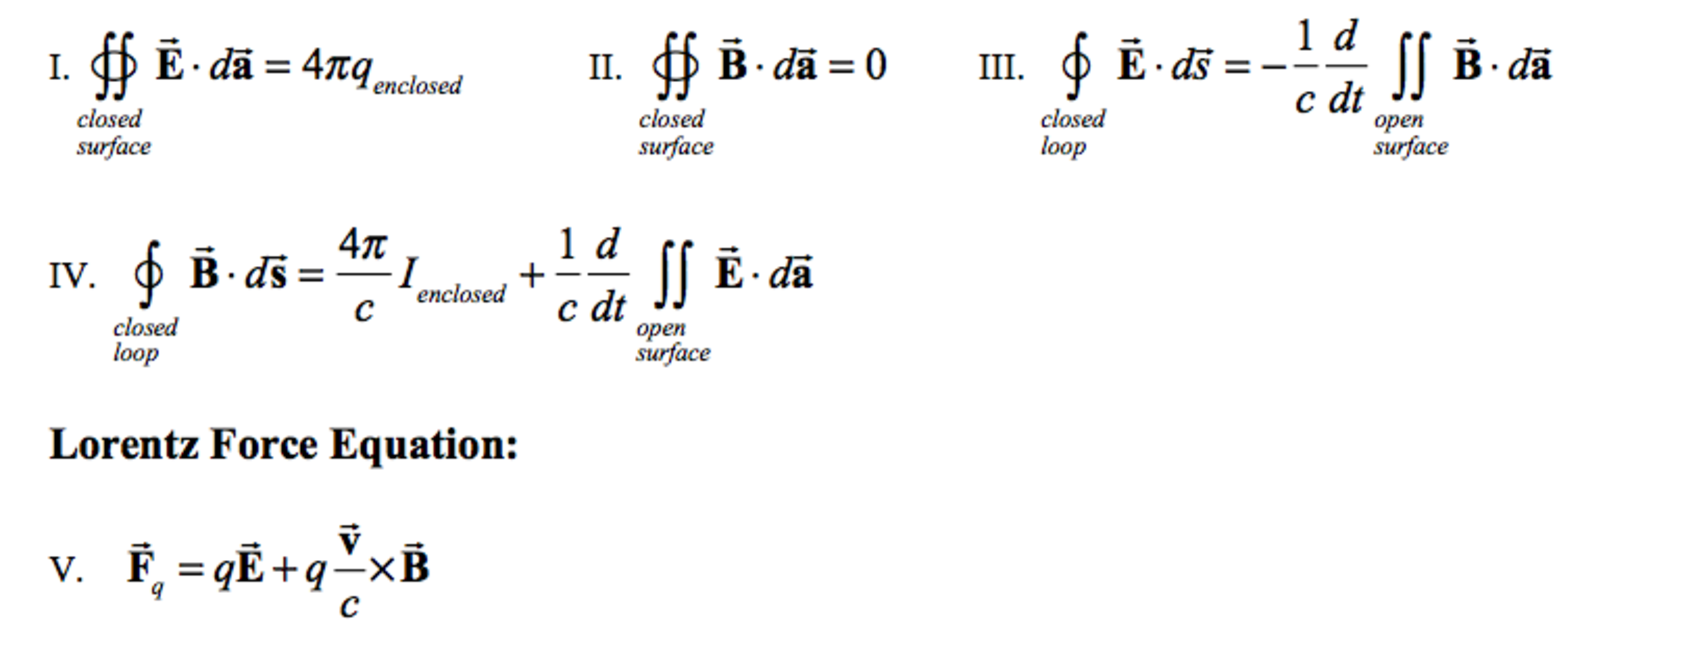
\includegraphics[width = 15cm]{eqns}
    \caption{Equations}
  \end{figure}
\begin{figure}[H]
    \centering
    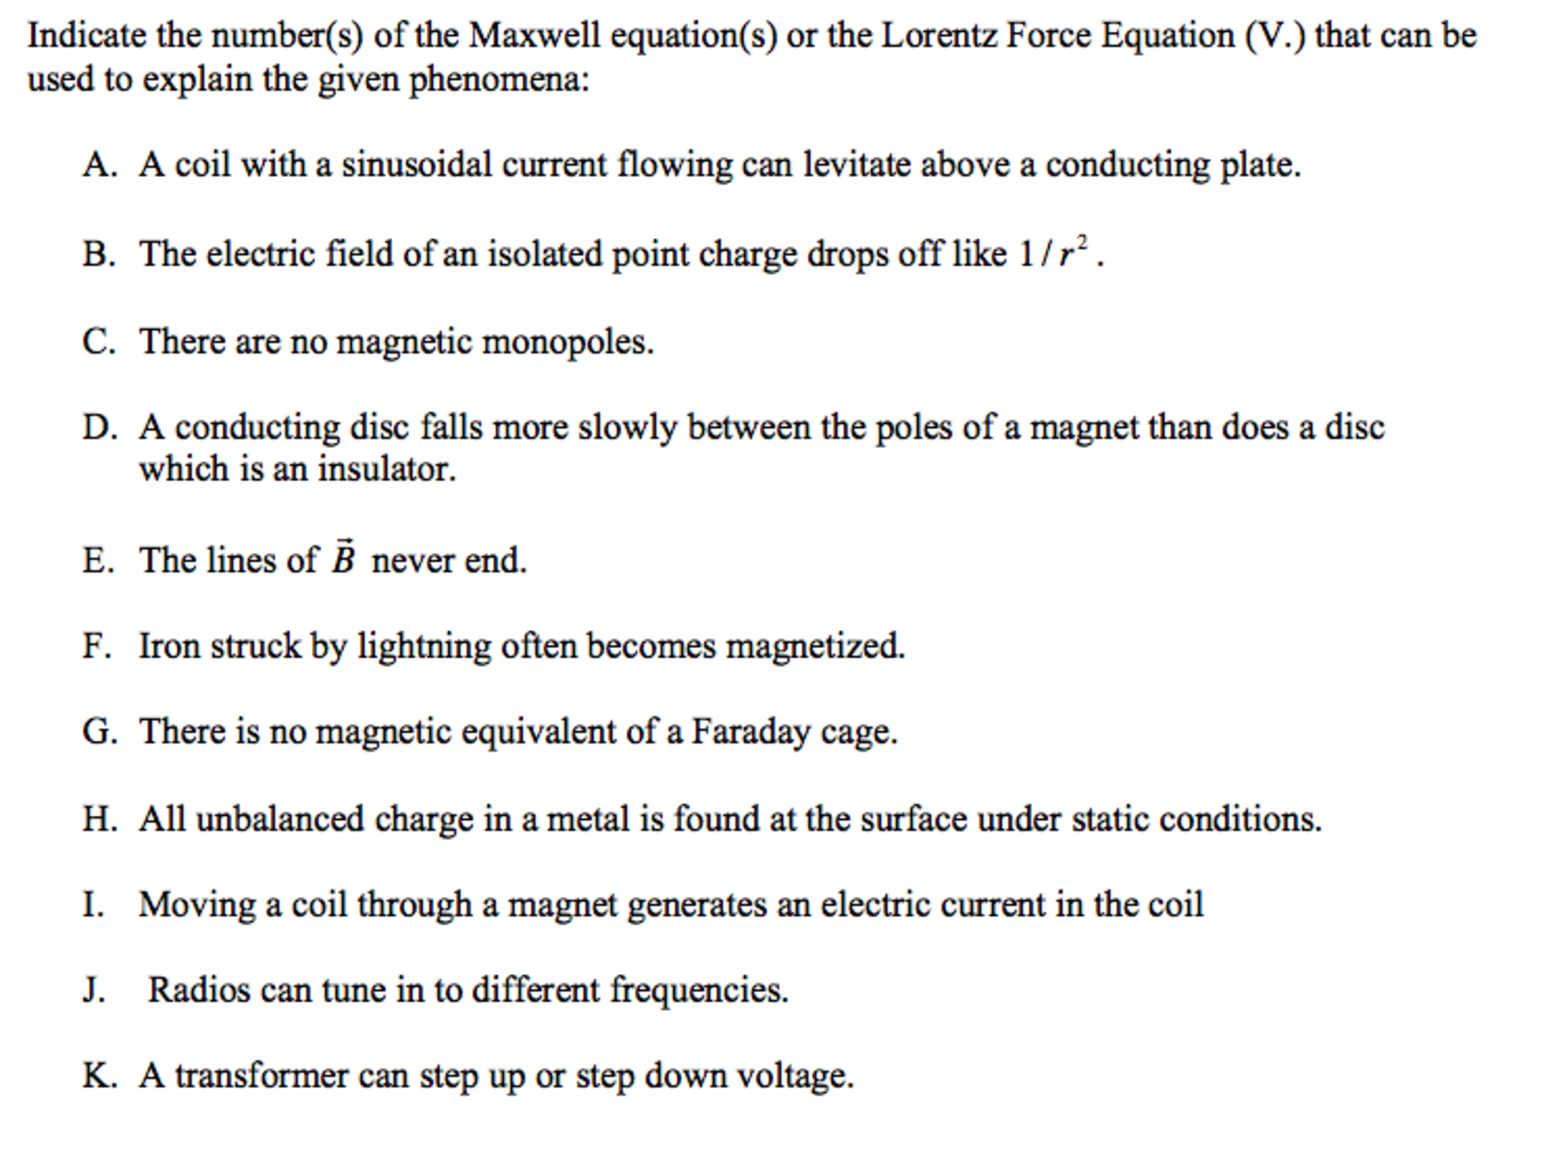
\includegraphics[width = 15cm]{max_gen}
    \caption{Maxwell's equations}
  \end{figure}
\section{Problem \thesection: Purcell 9.1}

\begin{figure}[H]
    \centering
    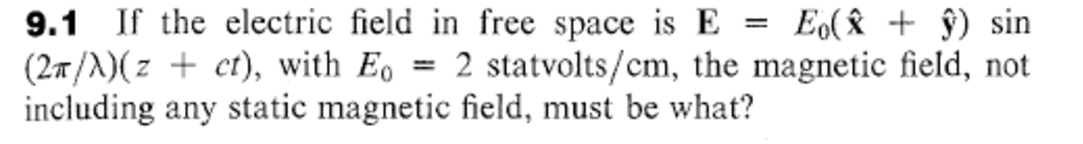
\includegraphics[width = 15cm]{pu901}
    \caption{Purcell 9.1}
  \end{figure}
  
\section{Problem \thesection: Purcell 9.5a}
 \begin{figure}[H]
    \centering
    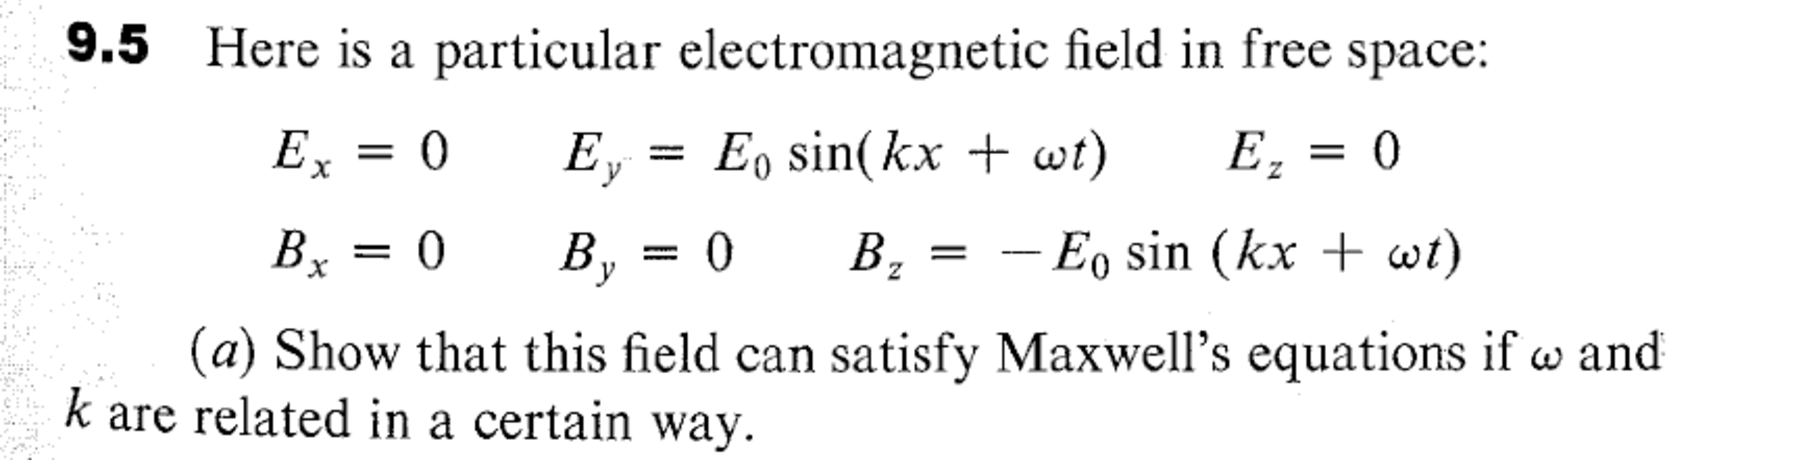
\includegraphics[width = 15cm]{pu905}
    \caption{Purcell 9.5}
  \end{figure}
\section{Problem \thesection: EM waves}
\begin{figure}[H]
    \centering
    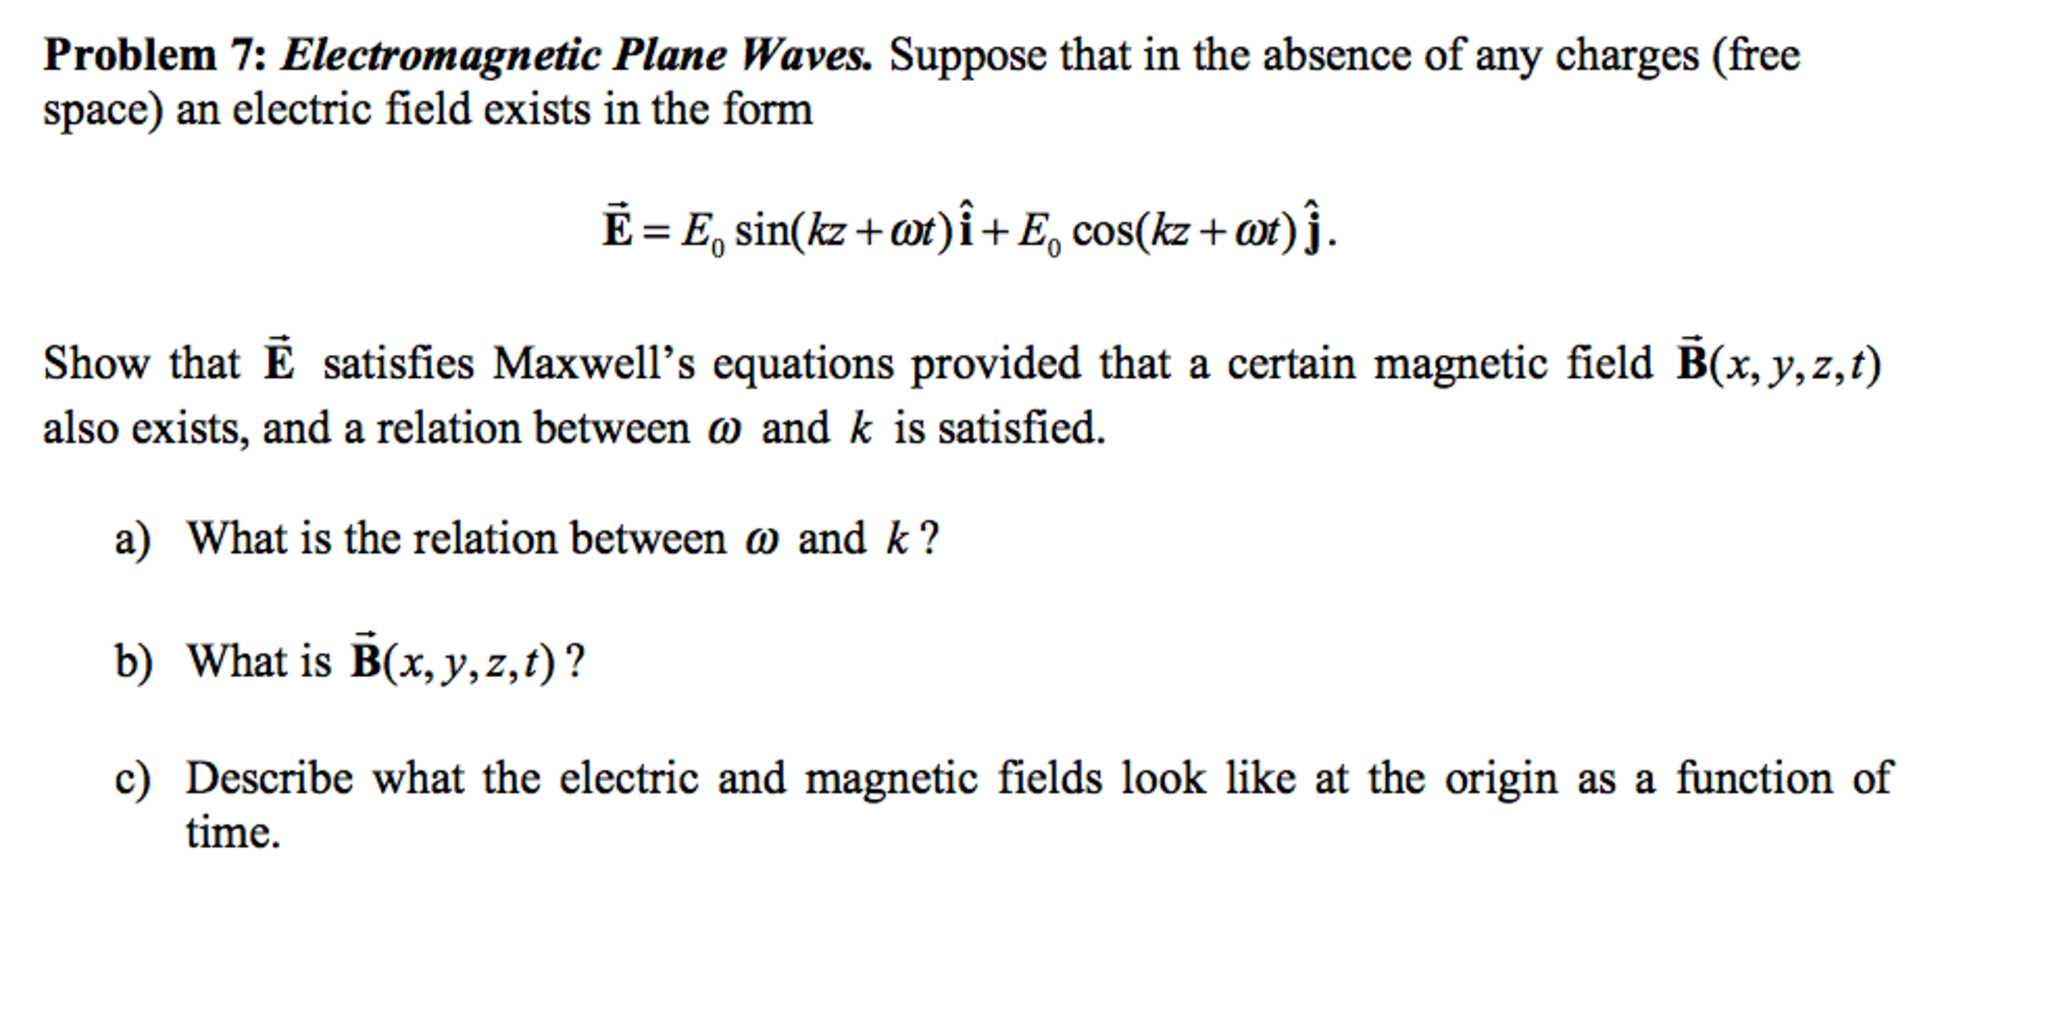
\includegraphics[width = 15cm]{waves2}
   \caption{Waves}
  \end{figure}
\section{Problem \thesection: Purcell 9.8}
\begin{figure}[H]
    \centering
    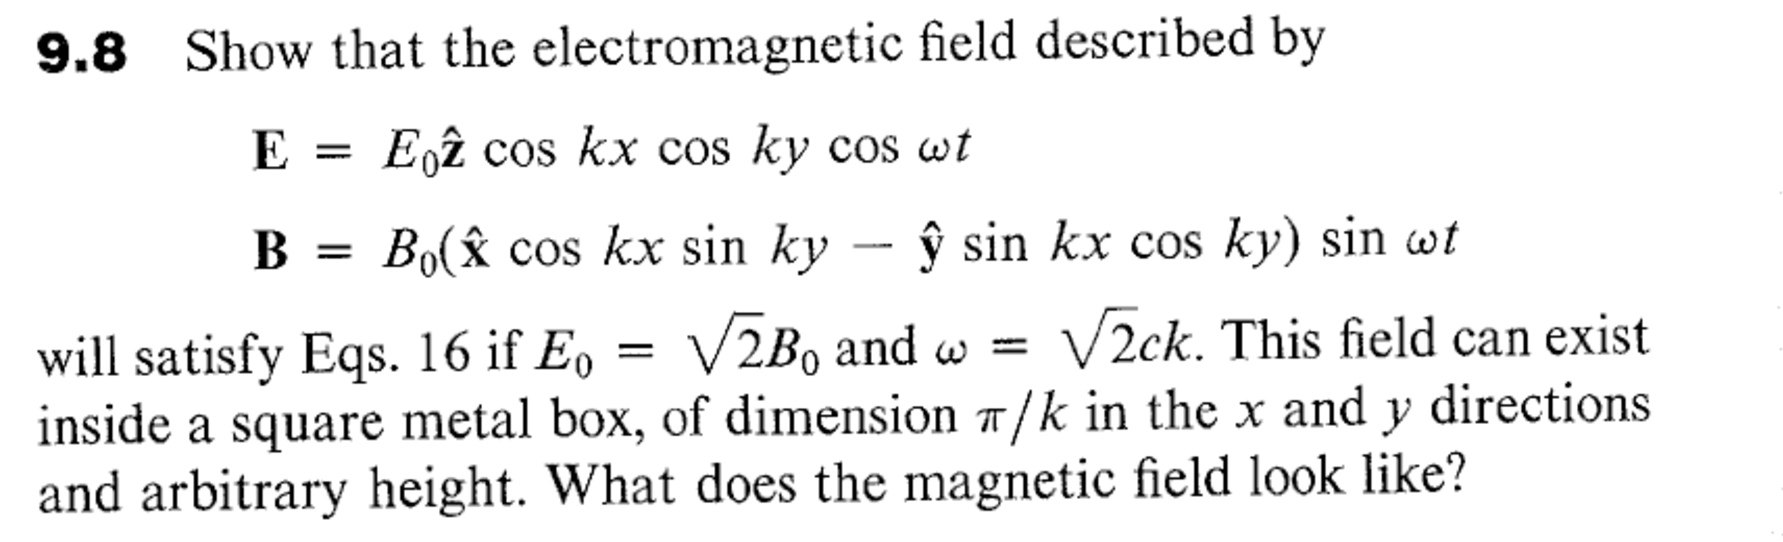
\includegraphics[width = 15cm]{pu908}
    \caption{Wave in a box}
  \end{figure}

\section{Problem \thesection: Galilean Transformation of Maxwell's Wave Equation}

Observers in frame $F$ take 8.022 and derive Maxwell's wave equation:
$$\nabla^2\vec{E} - \frac{1}{c^2} \frac{\partial^2\vec{E}}{\partial t^2} = 0$$
For simplicity and specificity, assume that $\vec{E} = E(x,t)\, \hat{y}$, and therefore, the wave equation reduces to:
$$\frac{\partial^2E}{\partial x^2} - \frac{1}{c^2} \frac{\partial^2E}{\partial t^2} = 0$$
The goal of this problem is to understand what form the wave equation would have for observers in another inertial frame $F'$ frame moving along the $x$ axis with speed $v$.  The Galilean transformation of coordinates between the two frames is:
$$x' = x - vt$$
$$t' = t~~~~~~~$$


\noindent
a. Use the chain rule to show that
$$\frac{\partial E}{\partial x} = \frac{\partial E}{\partial x'}$$


\noindent
b. Use the chain rule to show that
$$\frac{\partial E}{\partial t} = -v \frac{\partial E}{\partial x'} + \frac{\partial E}{\partial t'}$$


\noindent
c. Use the results of parts (a) and (b) to show that the original wave equation in $F$ transforms to
$$\frac{\partial^2E}{\partial x'^2} - \frac{1}{c^2} \frac{\partial^2E}{\partial t'^2} = -\frac{2v}{c^2} \frac{\partial^2E}{\partial x' \partial t'} + \frac{v^2}{c^2} \frac{\partial^2E}{\partial x'^2}$$
in frame $F'$.


\noindent
d. Show that in frame $F'$ a person computing the speed of waves, $V$, governed by the modified Maxwell wave equation, would find $V = v \pm c$.  You may simply assume that the waves are of the form
$$E(x' \pm Vt')$$
where $E$ is an arbitrary function.

\section{Problem \thesection: Optional: loop antenna}
\begin{figure}[H]
    \centering
    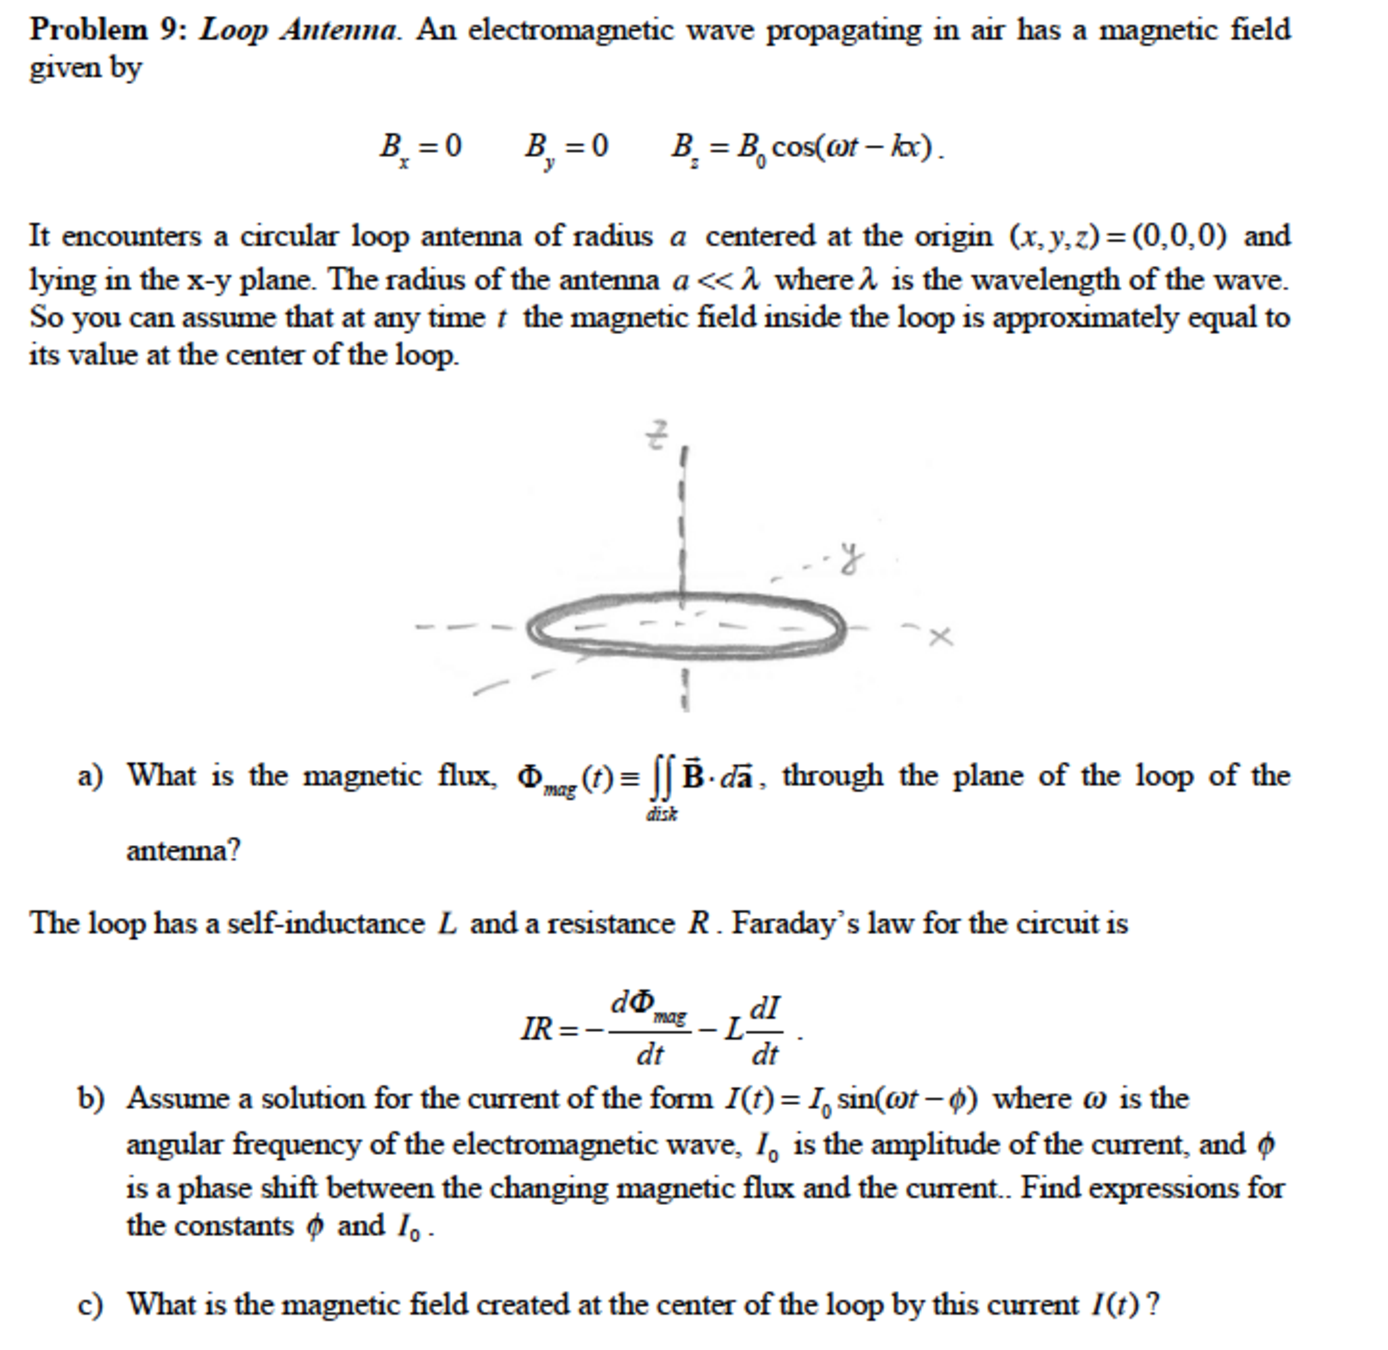
\includegraphics[width = 15cm]{loopantenna}
    \caption{Antenna}
  \end{figure}
\section{Problem \thesection: Optional --- Magnetic monopole: experiments}

 \begin{figure}[H]
    \centering
    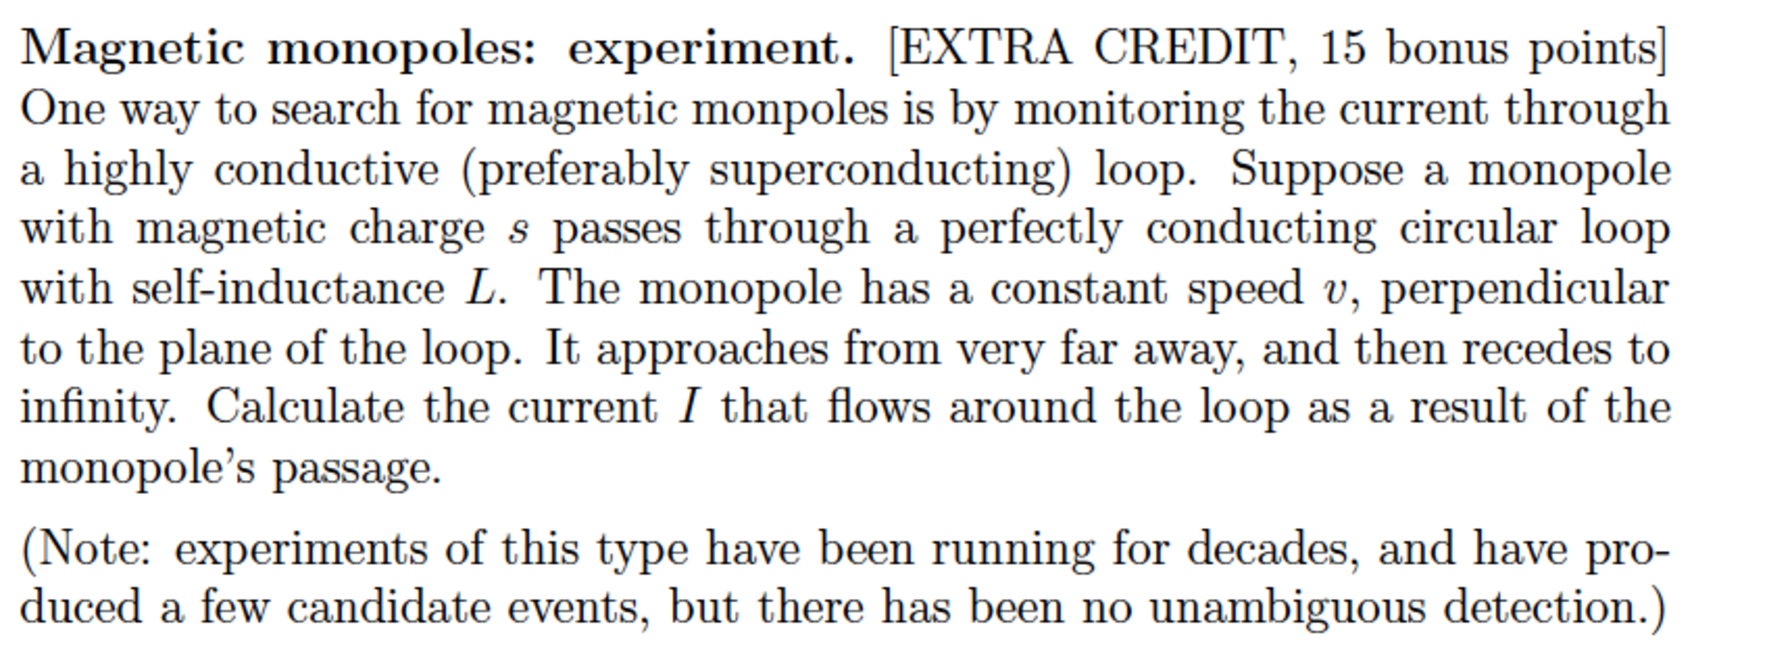
\includegraphics[width = 15cm]{monopoles}
    \caption{Magnetic monopole}
  \end{figure}

\section{Problem \thesection: The Director's Challenge --- Extra credit!!!}
  Formulate an interesting problem that relates a topic from 8.022 to your
  intended major or any other topic about which you are passionate.  Give references
  to help future students to understand the context.  Try to give a solution.
  Any method --- theoretical, analytical, numerical, experimental --- is acceptable.
  If you can't give a full solution, outline partial solutions. Enjoy!
\end{document}
